\chapter{Related Work}
\label{text:related}
Socially-aware and safe navigation among human pedestrians poses a problem which is far from being solved and applicable to a wide range of real-world scenarios. One of the challenging factors of this field lies in the broad palette of building blocks that a possible solution may depend on, each being a challenging subproblem. In the following, some of the related subproblems tackled within project \project are introduced.

\section{Pedestrian Prediction}
\label{text:related/prediction}
The problem of predicting human motions has been tackled by many different approaches. Some approaches try to model the human dynamics, including the dynamics of their interaction with their environment, or try to come up with a cost function that the human is trying to maximize (ontological methods). Other approaches model the pedestrian behavior merely by observing and (afterward) replicating it, without the use of inherent assumptions about the structure of the interaction or the human mindset itself (phenomenological methods).

\subsection{Ontological Approaches}
As described above, ontological approaches tackle the problem of predicting human movement by describing it as guided by an underlying "physical" model or some cost function. One popular example of a "physics-based" model, i.e., algorithms that model the pedestrian dynamics using first-order physical principles, is the social forces model \cite{Helbing1995}. The Social Forces model is one of the most commonly used pedestrian predictions models in the field, due to its combined capabilities to accurately predict the behavior of human movement, its interpretability, and its small computational complexity. The model uses first-order mechanical principles for forecasting the human motions in accordance with several interaction forces, that describe the impacts the pedestrian is exposed to:

\begin{align}
\vec{F} &= \underbrace{\frac{1}{\tau_{\alpha}} (v^0_{\alpha} \vec{e}_{\alpha} - \vec{v}_{\alpha})}_{F_{goal}} - \underbrace{\nabla_{\vec{r}_{\alpha \beta}} V_{\alpha \beta}[b(\vec{r}_{\alpha \beta})]}_{F_{interaction}} 
\label{eq:social_forces} \\
2b &= \sqrt{(||\vec{r}_{\alpha \beta}|| + ||\vec{r}_{\alpha \beta} - v_{\beta} \dt \vec{e}_{\beta}||)^2 - (v_{\beta} \dt)^2}
\end{align}

For every pedestrian $\alpha$, Social Forces describes an attractive force to reach an imaginary goal position with desired velocity $v^0_{\alpha} \vec{e}_{\alpha}$, with $\vec{e}_{\alpha}$ being the unit direction vector pointing from the pedestrian's current to its goal position and $v^0_{\alpha}$ being the desired speed, e.g.,\ the maximal speed. The second force describes the repulsive forces the pedestrians exert among each other, modeled by the gradient of some potential field $V_{\alpha \beta} = V_{\alpha \beta}^0 \exp(-b / \sigma)$ in the direction pointing from pedestrian $\alpha$ to pedestrian $\beta$. Thereby, $b$ takes the relative speed and directions of the regarded pedestrian pair into account. While Social Forces is a mainly deterministic model, similar approaches use recursive Bayesian filtering to deal with uncertainty, such as \cite{Schneider2013}\cite{Rehder2015}\cite{Guo2016}. Due to the small computational complexity and the high interpretability of these models, they tend to be very useful for large scale simulations but are prone to modeling errors in small scale predictions, as they widely hinge on a set of estimated parameters which is assigned individually to each pedestrian, might not grasp the exact dynamical model of the pedestrian and do not take into account knowledge about past interactions, which is likely to be important for the up-coming interactions.
\newline
Another way of explicitly formulating the humans' interaction with their environment is by deriving a cost function that the human maximizes during the interaction. While some works describe the cost function as a payoff of a cooperative or adversarial game and apply game theory to predict the behavior of the other agents as well as of the agent itself, such as \cite{Bouzat2014}\cite{Nikolaidis2017}, other works use \ac{IRL} \cite{Ng2000} to characterize the interaction as a value function assigned to each state-action-pair, such as \cite{Fahad2018}\cite{Fernando2019}\cite{Saleh2018}, or as an expansion to probabilistic predictions using maximum entropy \ac{IRL} \cite{Ziebart2008}. Since IRL-based approaches rely on the Markovian property, they are not capable of including the interaction history while losing the property of interpretability by using a sufficiently complex reward function for modeling human interaction. Consequently, these approaches might work well under the constraints of limited data due to the possibility of encoding prior knowledge and the extrapolation capabilities of \ac{IRL}-based approaches but lack behind phenomenological in the presence of many available data.

\subsection{Phenomenological Approaches}
Phenomenological methods incorporate data-driven techniques to observe and imitate human behavior. As a consequence, they make merely minimal assumptions about the inherent interaction process, especially in comparison to most of the ontological methods discussed above. Therefore, the availability of a reasonably large set of observable data is the key to developing a well-performing prediction model. However, since increasingly many pedestrian datasets became available over recent years, such as \cite{Pellegrini2009}\cite{Rasouli2019}\cite{Caesar2020}, phenomenological models became increasingly accurate for a wide range of scenarios. 
\newline
In contrast to previously described methods, phenomenological approaches do not assume Markovian state transitions and are therefore capable of taking the state histories of each agent into account, a presumably crucial feature for a precise prediction over future states. \ac{LSTM} modules \cite{Hochreiter1997} have been developed to model temporal sequences and are thus perfectly suitable for the purpose of mining past human trajectories for predicting future states, as done in \cite{Chen2019a}\cite{Hug2018}\cite{Zhang2019}\cite{Jain2016} (similarly using GRUs \cite{Liu2020}). However, the resulting deterministic trajectory output is not able to account for the uncertainty assigned to each prediction of future states, particularly due to the dynamic nature of human gait. To fully account for each possible future outcome, however, unimodal predictions would either miss some eventualities or be overly conservative estimates. 
\newline
Generative models proved to be well applicable to solve this dilemma by producing general (including multi-modal) probability distribution over future pedestrian trajectories, learned from data. A \ac{GAN} \cite{Goodfellow2014}, a type of (deep) generative models, has been widely used in the field, as in \cite{Gupta2018}\cite{Kosaraju2019}\cite{Ouyang2018} but is especially hard to train due to the internal conflict between generator and discriminator and generally output empirical distributions. Related to \ac{GAN}s are \ac{VAE}, a class of generative models that make use of a latent space. Conditional VAEs (CVAEs) have been recently used to predict distributions over pedestrian trajectories. CVAEs can learn the probability distribution of their latent space variables and map samples of these distribution to obtain a desired output distribution, allowing empirical as well as analytical distributions, and being easier to train in comparison to \ac{GAN}s. Especially, this only allows to formulate the desired output distribution to be processable for online usage. Examples of works using (C)\ac{VAE}s in the area of pedestrian prediction are \cite{Ivanovic2018}\cite{Salzmann2020}\cite{Poibrenski2020}\cite{Lee2017}.

\subsection{Trajectron}
The Trajectron++ model \cite{Salzmann2020} by Salzmann et alt., an enhancement of the original Trajectron model \cite{Ivanovic2018}\footnote{For the sake of brevity in the following the Trajectron++ model will be addressed by the Trajectron model.}, is a generative, graph-structured, pedestrian prediction model based on a C\ac{VAE}. By incorporating the state histories of various agents in the scene as well as their environment, it can efficiently predict a distribution over a full trajectory of future states, each being multi-modal and represented by a \ac{GMM}. Especially, to the best of the authors' knowledge, the Trajectron model is the only model within the field of pedestrian prediction that is able to condition the prediction on a robot's planned trajectory.

\begin{figure}[!ht]
\begin{center}
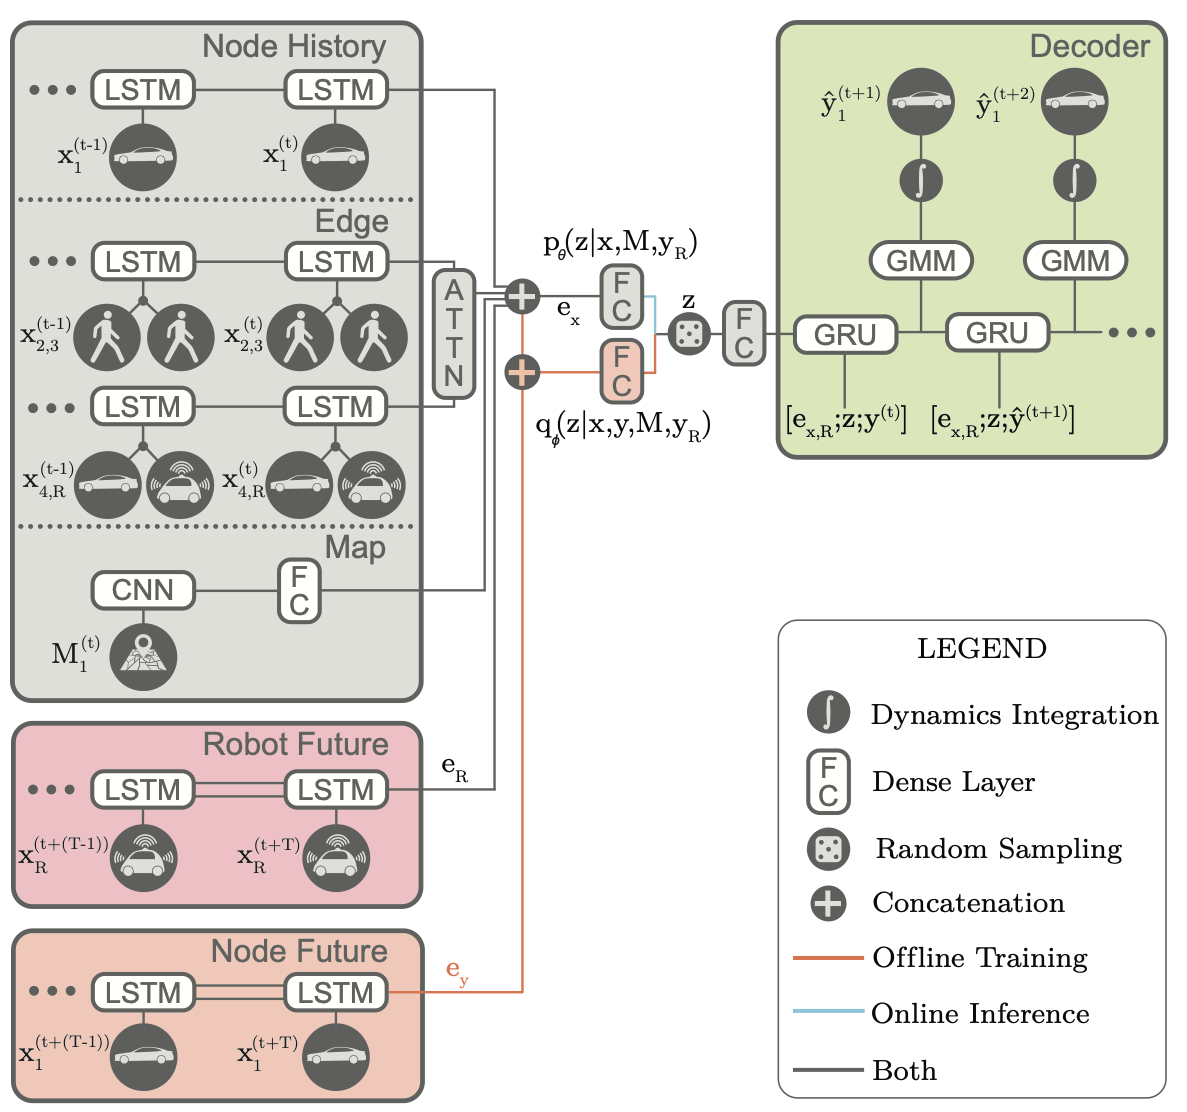
\includegraphics[width=\imgwidth]{images/trajectron++.png}
\captionof{figure}{Spatiotemporal network architecture of Trajectron++ model \cite{Salzmann2020}}
\label{img:trajectron_model}
\end{center}
\end{figure}

\begin{equation}
\max_{\phi, \theta, \psi} \sum_{i=1}^N \mathbb{E}_{z \sim q_{\phi}(z | x_i, y_i)} [\log p_\psi (y_i | x_i, z)] - \beta D_{KL} (q_{\phi}(z | x_i, y_i) || p_{\theta}(z | x_i)) + \alpha I_q(\boldsymbol{x}; z)
\label{eq:trajectron_loss}
\end{equation}

Figure \ref{img:trajectron_model} shows the architecture of the Trajectron model. Each agent in the scene is modeled as a node in a spatio-temporal graph, with assigned state history and properties shared by nodes of the same type, e.g.,\ pedestrian or vehicle. Equation \ref{eq:trajectron_loss} shows the loss function the model is being trained with. In the first step, the inputs, which are the state history of each node, including the robot, the environment obstacle map, as well as the planned robot trajectory (inputs $\boldsymbol{x}$), are encoded to a 25 dimensional latent space $\boldsymbol{z}$. The latent space representation is then sampled to generate the output distribution $\boldsymbol{y}$, unrolled over the full prediction horizon. Formally, the model is described as estimating the conditional probability distribution $p(\boldsymbol{y}|\boldsymbol{x})$ by marginalizing over the latent variable $\boldsymbol{z}$:

\begin{equation}
p(\boldsymbol{y}|\boldsymbol{x}) = \sum_{\boldsymbol{z}} p_{\psi} (\boldsymbol{y} | \boldsymbol{x}, z) p_{\theta}(z | \boldsymbol{x})
\end{equation}

The optimization can be regarded as maximizing the $\beta$-weighted evidence lower-bound of the conditional distribution $p(\boldsymbol{y}|\boldsymbol{x})$ \cite{Ivanovic2018}. Although the model is able to deal with the agent's environment as well as several types of agents project, \project focuses on the pedestrian type in a free-space environment, which is described in Section \ref{text:approach/formulation} and its implications in Section \ref{text:experiments/integration}.

\section{Safe Planning under Uncertainty}
\label{text:related/uncertainty}
Trajectory optimization itself is a wide field with many different methodologies. Though the area can be roughly broken down into two categories, shooting and collocation \cite{Kelly2017}.\footnote{There are several other directions of separation possible such as the direct vs indirect methods, but I will focus on shooting vs collocation here. Further information about the taxonomy of trajectory optimization can be found in \cite{Kelly2017}  and \cite{Chai2020}.} Shooting optimizes for the control inputs and unrolls them using a simulation environment to compute objective and constraint. Thereby, the dynamics constraint $x = \f(x, u)$ is intrinsically enforced. In comparison, collocation uses all controls and states as decision variables while constraining the system dynamics and tries to solve the \ac{NLP} by approximating some function (e.g.\ Lagrange polynomials in orthogonal collocation).
\newline
While traditionally, the problem of trajectory optimization under uncertainty has been tackled by using fixed error bounds on all uncertainties in the system, which is also known as robust control \cite{Bemporad1999}. Consequently, solutions obtained were largely sub-optimal due to widely overestimating the actual system uncertainties, or the optimization formulation became infeasible and thus impossible to solve. Subsequently, many different directions of research have evolved, such as formulating the problem as a \ac{POMDP} and (online) \ac{POMDP}-solvers to find feasible trajectories \cite{Chen2016}, using Monte-Carlo planning \cite{Janson2015} \cite{Silver2010}, signal temporal logic \cite{Sadigh2016}, (probabilistic) decision graphs \cite{Koenig1994}, sampling-based methods, as well as constraint formulations that estimate and bound the risk (or chance) of collision \cite{Ono2015}\cite{Lew2019}\cite{Chow2015a}\cite{Chow2013}\cite{Ono2012}\cite{Ludersa}\cite{Luders2011}\cite{Otte2014} or reachability-based concepts for guaranteeing the impossibility of collision solely on the base of the dynamical properties and initial conditions of interacting agents \cite{Leung2020}\cite{Dhinakaran2017}\cite{Margellos2009}\cite{Chen2017b} \cite{Althoff2009}\cite{Althoff2010}. Since discussing all of these different techniques surely is out of the scope of this work, only three approaches, which are most relevant to this work, will be examined in the following:

\subsection{Sampling-based Path Planning}
Sampling-based path planning methods, such as RRT \cite{LaValle1998}, have been shown to be an efficient solution for path planning in continuous-space, static environments, while often guaranteeing asymptotic optimality and feasibility of the derived solution, such as \cite{Karaman2011}\cite{Luders}. These algorithms are iteratively sampling random points from the configuration space, while retaining those in the free space (i.e., free from obstacles), storing them as milestones in a roadmap, and connecting those milestones, which can be connected completely in the free space. The algorithm repeats until either the goal state has been incorporated in the roadmap or the maximal computation time has exceeded. To account for dynamic and probabilistic obstacles, a temporal dimension has to be added to the search space, making the problem computationally challenging to solve in real-time. For addressing this issue, rapid replanning and repairing \cite{Otte2014} are often used. To implicitly take into account system uncertainties, the occupancy cost can be augmented by risk level sets that assign a certain risk to each robot state, depending on the obstacle's state, e.g., its orientation and velocity, as shown in \cite{Pierson2018}\cite{Pierson2019}. However, despite the success of sampling-based methods in online path planning, they do not explicitly leverage future predictions of the environment and are therefore restricted to only (temporally) locally optimal solutions.

\subsection{Chance Constraints}
Chance constraints are a specific way of formulating a constraint under uncertainty, such that it holds for at least a pre-defined probability level $p$. With a general inequality constraint $g(x) \leq 0$ it is:

\begin{equation}
Pr(g(x) \leq 0) \geq p
\label{eq:chance_constraint}
\end{equation}

Usually, constraint \ref{eq:chance_constraint} is reformulated as a set of deterministic constraints to be manageable for optimization. Therefore, several methods have been purposed: Sampling-based methods relying on the Bernstein approximation \cite{Calafiore2005}, on scenario planning approach \cite{Bemporad1999}, or Monte Carlo sampling \cite{Hong2011}\cite{Janson2015} as well as dynamic-programming based approaches for discrete space \cite{Chow2013}\cite{Ono2015} \cite{Chow2015a}. While these methods work for general distributions but are usually too slow for an online optimization approach, shrinking the space of distributions can improve the performance, such as in \cite{Chen2018}\cite{Calafiore2006}\cite{Carvalho2014}\cite{Blackmore2009}\cite{Blackmore2011}. Thereby, handling multi-modality of the risk distribution efficiently is a widely untouched ground, to the best of the authors' knowledge, which only has been solved for a specific scenario, such as in \cite{Hu2018}. To conclude, solving a chance constraints program efficiently is quite hard to do, especially when dealing with general, such as multi-modal and non-convex risk distributions.

\subsection{Hamilton-Jacobi Reachability} 
Reachability analysis deals with the problem of a two-person, zero-sum differential game. Specifically, it tries to solve the question how to react if there is another player that interferes with the fulfillment of the robot's objective by optimizing the joint system state, assuming that the counter-player always counters the robot's action optimally, i.e., assuming the worst case disturbance $\d = \beta[\u]$ \cite{Pavone2020}. Under these conditions, the optimal control strategy can be derived by maximizing: \\

\begin{equation}
V(x(t), t) = \min_{\beta[\u](\cdot)} \max_{\u(\cdot)} \left[ \int_t^0 l(\x(\tau), \u(\tau), \boldsymbol{d}(\tau)) \, d\tau + l_f(\x(0)) \right]
\label{eq:j_reachability}
\end{equation}

with $(\x(\tau), \u(\tau), \d(\tau))$ describing the joint system with dynamics $f(\boldsymbol{x}, \u, \d)$. While solving the robot's optimal control strategy $\u_{opt}$ in open-loop (also \textit{forward} reachability) is computationally inexpensive but leads to overly conservative and hence un-realistic estimates, since the counter-player knows the entire policy $\u_{opt}$ in advance and can re-act accordingly, \ac{HJR} (also \textit{backward} reachability) addresses the problem of maximizing Equation \ref{eq:j_reachability} in closed-loop, i.e., by allowing the robot to adapt its control policy at each time-step. As proven in \cite{Pavone2020}, this is equivalent to solving the Hamilton-Jacobi-Isaacs differential equation with boundary condition: \\

\begin{problem}{General \ac{HJR} problem}
\begin{align}
\pd{V}{t} + \max_{\u}  \min_{\d} &\left[l(\x, \u, \d) + \nabla V^T f(\x, \u, \d) \right] = 0 \\ 
V(\x, 0) &= l_f(\x) \\
\Rightarrow \u_{opt} &= \arg \max_{\u}  \min_{\d} \nabla V^T f(\x, \u, \d)
\label{eq:hjr_problem_u}
\end{align}
\label{eq:hjr_problem}
\end{problem}

Solving Problem \ref{eq:hjr_problem} has been examined for several scenarios and applications over the recent years, as in \cite{Dhinakaran2017}\cite{Margellos2009}\cite{Chen2017b}, and has shown to be especially useful in the field of autonomous driving \cite{Althoff2009}\cite{Althoff2014}\cite{Althoff2010}. In opposite to forward reachability, \ac{HJR} finds the non-overly conservative avoidance maneuvers, "stemming from its equivalence to an exhaustive search over the joint system dynamics" while still being flexible with respect to the system dynamics, as depicted by \cite{Leung2020}. To solve \ref{eq:hjr_problem}, the value function $V(\cdot)$ as well as its gradient are computed for every cell of a $n$-dimensional grid that discretizes the joint state $\x(\tau)$ and for some discrete time horizon (including $\tau \rightarrow \infty$). 

\section{Navigation in Human Crowds}
\label{text:related/crowd_navigation}
Navigation in human crowds is especially important for vastly integrating autonomous ground vehicles in our daily life but poses a hard problem due to a priori unknown human intentions and hard to quantify objectives, e.g.,\ the notion of socially-acceptable behavior. Existing work in this field can be roughly divided into two main directions, model- and learning-based approaches: 

\subsection{Model-Based Approaches}
Traditionally, the pedestrians are regarded as dynamic obstacles, with the collision avoidance algorithm being used for robot navigation \cite{vandenBerg2011}\cite{Fox1997}\cite{Luo2018a}\cite{Phillips2011}. \ac{ORCA} \cite{vandenBerg2011}, for example, guarantees a collision-free pre-defined time horizon, under the assumption of perfect knowledge about the state of each interacting agents as well as, more importantly, a shared, deterministic policy over all agents. Although these models have been advanced to relax some of the assumptions such as perfect perception \cite{Hennes2012}, they still fail to capture a human-like behavior and, consequently, may lead to unsafe and socially unacceptable robot actions. To solve this issue, it is crucial to directly include the predicted impact of the robot's planned trajectories into the optimization itself. For this reason, the robot's motion has been incorporated in some of the (model-based) pedestrian prediction models discussed in Section \ref{text:related/prediction}, e.g.,\ the Social Forces model \cite{Helbing1995}, usually by augmenting the model by robot-specific parameters while preserving the general concept of interaction \cite{Ferrer2013}\cite{Luo2018a}. Nonetheless, as discussed, these models usually are largely hinging on parameters, making them hard to tune and hence inaccurate in prediction and thus planning as a consequence of modeling errors. Additionally, model-based approaches are usually deterministic, regarding only one out of assumably many possible outcomes, and therefore might lead to un-safe behavior.

\subsection{Learning-based Approaches}
Learning-based approaches try to replicate human behavior that has been learned from human demonstration in simulations or by accumulating features over possible trajectories of interacting agents while minimizing some interactive cost function (e.g.,\ the separation distance) \cite{Kim2016}\cite{Kretzschmar2016}. While these models tend to plan trajectories that are more socially acceptable and natural, they are much larger in computational cost and very hard to train due to the dynamic and stochastic nature of human gait. Other approaches come up with a set of socially compliant rules, such as "passing on the right" and use deep reinforcement learning to apply them  \cite{Knepper2012}\cite{Chen2017}\cite{Everett2018}. However, it can be doubted whether these methods can be generalized to unseen scenarios, how to certify a safe interaction, and whether these rules hold at all.
\newline\newline
While model-based approaches are computationally efficient and traceable but lack an accurate capturing of human behavior, learning-based methods do model the human motion more naturally and are therefore capable of planning socially-aware trajectories. However, they tend to be computationally expensive, are neither interpretable nor able to give any safety guarantees, which is crucial for secure human-robot interaction. Therefore, this works wants to combine both worlds, the predictive abilities of deep learned models with the safety guarantees of model-based safety guaranteeing methods, such as \ac{HJR}, which was discussed above. To truly leverage the full "knowledge" of the prediction model, concepts of model-gradient informed concepts, which have been already shown to be successful in control theory \cite{Chen2019}\cite{Fan2020}, are thereby re-formulated for trajectory optimization. While most of the described approaches deal with deterministic and uni-modal predictions, due to the highly stochastic human motion, anticipatory and efficient, but safe interactions can only be derived when the system can reason about many possible future outcomes of the scenario so that multi-modality should be taken into account.

% sequential-action control \cite{Nishimura2020}\cite{Nishimura2020a}